\documentclass[11pt]{scrartcl} 
\usepackage[utf8]{inputenc}
\usepackage{tikz}
\pagenumbering{gobble}


\begin{document}

\begin{figure}
\resizebox {.8\textheight} {!} {
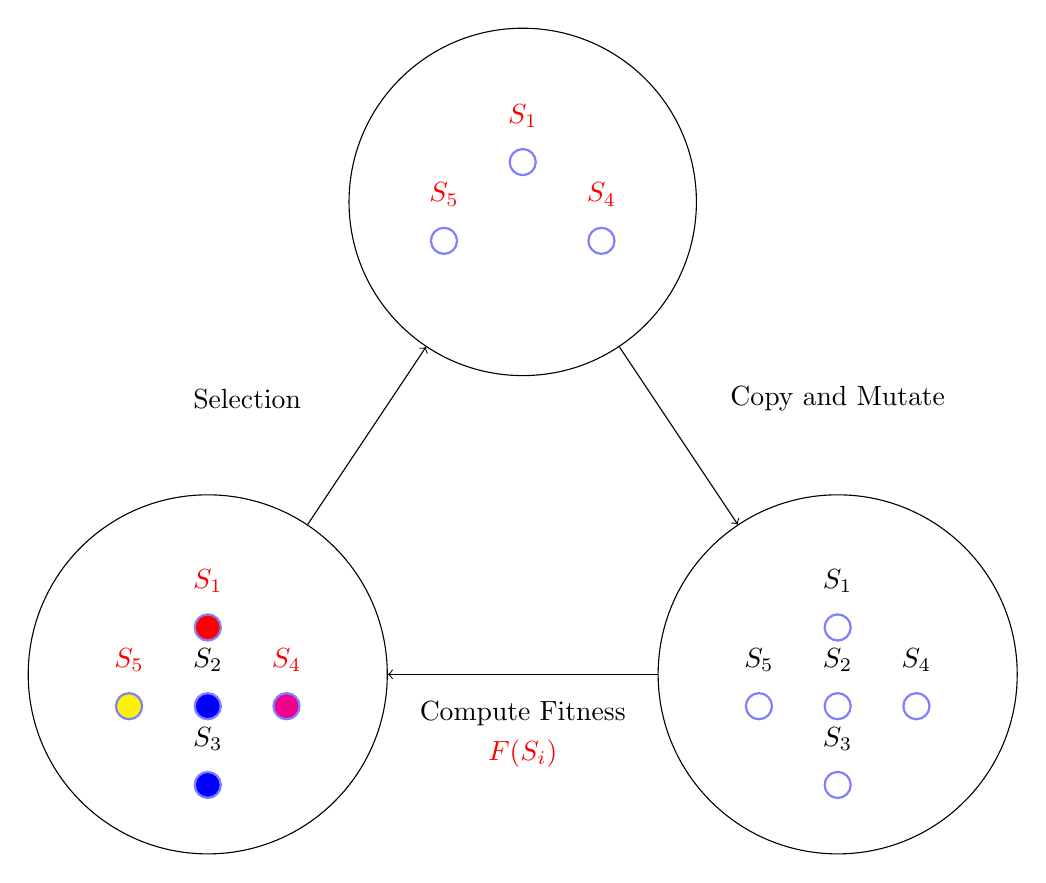
\begin{tikzpicture}[sequence/.style={circle,draw=blue!50,fill=white!20,thick}, node distance = 10cm]
    \node (A) at (0,0) [matrix, draw, shape=circle]  {
	\node (s1) at ( 0,2) [sequence] {};
	\node (s2) at ( 0,1) [sequence]  {};
	\node (s3) at ( 0,0) [sequence]  {};
	\node (s4) at ( 1,1) [sequence]  {};
	\node (s5) at ( -1,1) [sequence]  {};
	
	
	\node [black, above] at (s1.north) {$S_1$};
	\node [black, above] at (s2.north) {$S_2$};
	\node [black, above] at (s3.north) {$S_3$};
	\node [black, above] at (s4.north) {$S_4$};
	\node[black,above] at (s5.north) {$S_5$};
     ; \\
    };
    \node (B) at (-8,-0) [matrix, draw, shape=circle] 
    {
  	\node (s1) at ( 0,2) [sequence, fill=red] {};
	\node (s2) at ( 0,1) [sequence,  fill=blue]{};
	\node (s3) at ( 0,0) [sequence, fill=blue]{};
	\node (s4) at ( 1,1) [sequence,  fill=magenta]{};
	\node (s5) at ( -1,1) [sequence,  fill=yellow]{};
	
	
	\node [red, above] at (s1.north) {$S_1$};
	\node [black, above] at (s2.north) {$S_2$};
	\node [black, above] at (s3.north) {$S_3$};
	\node [red, above] at (s4.north) {$S_4$};
	\node[red,above] at (s5.north) {$S_5$};
       ;\\
    };
    
     \node (C) at (-4, 6) [matrix, draw, shape=circle]{
     	\node (s1) at ( 0,2) [sequence] {};
	\node (s4) at ( 1,1) [sequence]  {};
	\node (s5) at ( -1,1) [sequence]  {};
	
	
	\node [red, above] at (s1.north) {$S_1$};
	\node [red, above] at (s4.north) {$S_4$};
	\node[red,above] at (s5.north) {$S_5$};

       ;\\
    };    
    \draw [->] (A) edge (B) (B) edge (C) (C) edge (A);
    \draw (-4, -0.5) node {Compute Fitness};
    \draw [red] (-4, -1) node {$F(S_{i})$};
    \draw (-7.5, 3.5) node {Selection};
    \draw (0, 3.5) node {Copy and Mutate};
    

    
\end{tikzpicture}
}
\end{figure}

\end{document}
